An important role of an experiment in organ-on-a-chip applications, as well as the whole biomedical field, is given by the video analysis. In fact, analyze the video just one time in real-time, during the experiment is running is never sufficient. So, what the system described in this thesis needs to be usable, is a way to memorize the video in order to be used, watched, in a second time.

To fulfill this aim I designed a console application using the \textit{Qt} framework. The motivation that brought me to use this framework is that the same code can run in different platform. In other words, this application can run on \textit{Linux}, \textit{Windows}, and \textit{MacOS}  indistinctly. This is a big advantage, because in a laboratory environment there are many researchers, and it is very easy to encounter different operating systems.

 In (App.\ref{code:video}) the listings of this application are shown. As can be seen, the source codes are divided in such a way to ensure high hierarchical efficiency.
 
 Indeed, the main (List.\ref{code:mainstoring}) of this application just instantiates a \textit{MyTimer} object. This \textit{MyTimer} object (List.\ref{code:timer}) is in charge to generate an interrupt every $10\ sec$, and it starts from its creation. When this interrupt comes, the timer uses the \textit{Downloader} object to check if  a new microscope video has been uploaded, and if so, download it and reset the flag that points up the new video status. The code of \textit{Downloader} is shown in (List.\ref{code:downloader}). The videos are stored inside the directory \textit{C:/Video} and their names correspond to the date and hour of download. 
 
 \begin{figure}[h]
 	\centering
 	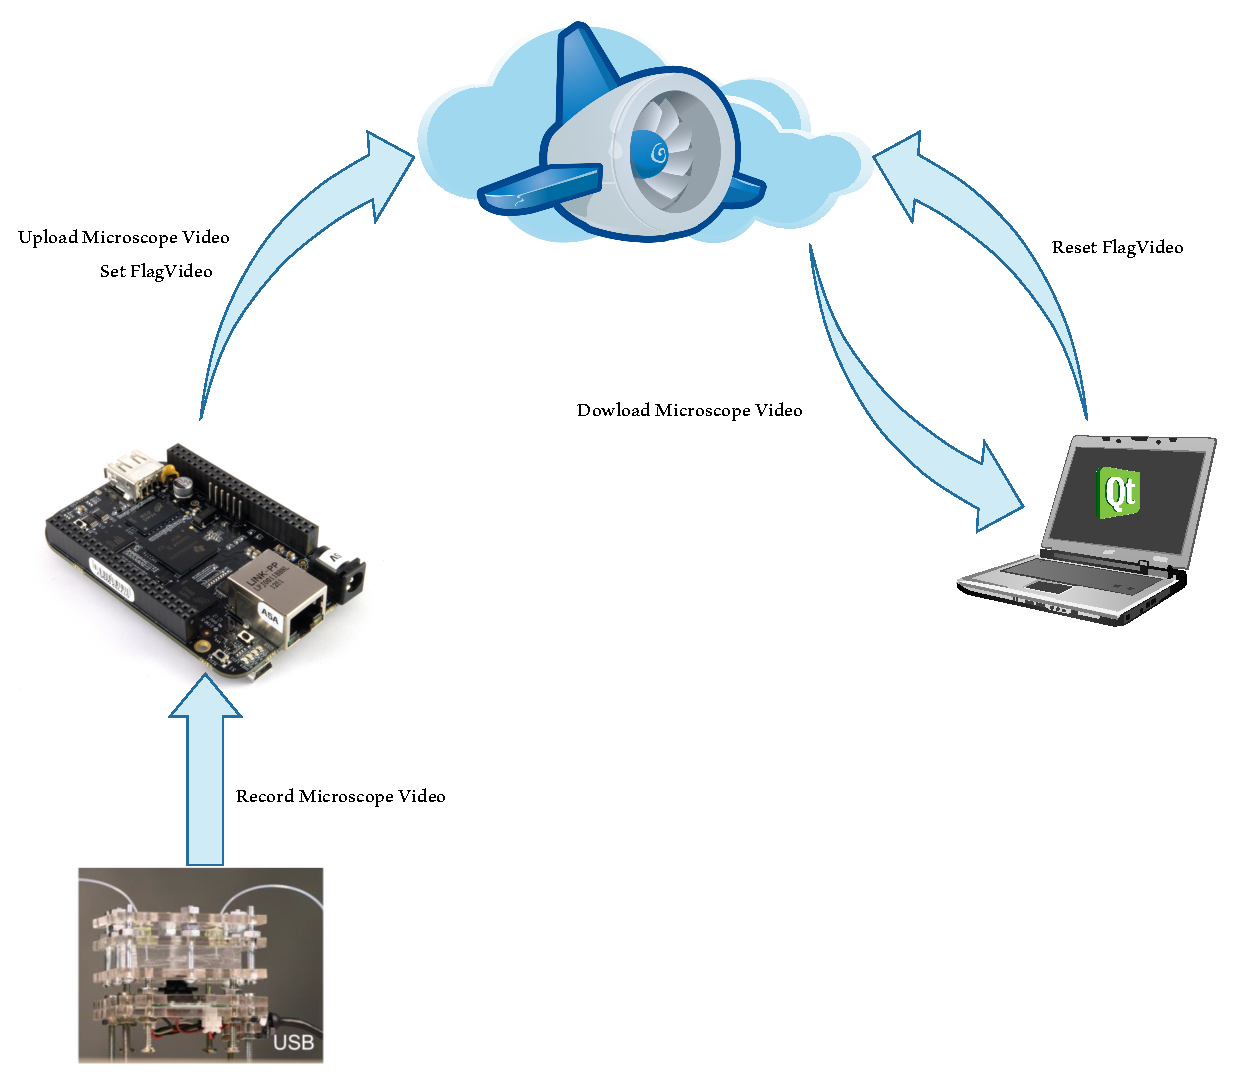
\includegraphics[width=\textwidth]{storing/videostoring}
 	\caption{Video Storing: Block Diagram}
 	\label{Fig:videostoring}
 	
 \end{figure}
 
 The (Fig.\ref{Fig:videostoring}) shows the basic step in which the microscope video is stored. Once the Beaglebone Black has recorded the microscope video, this is upload onto Google App Engine by the board itself, and then the \textit{video flag} is asserted in order to advice the Video Storing application that a new video has been uploaded. Finally, the application downloads and stores this video inside the computer hard drive and resets the flag.
 
 The (List.\ref{code:pro}) shows the taken decision to do not use the graphic user interface (\textit{GUI}) for this application, in order to lighten the application itself, and to allow the use of network.
 
  \begin{figure}[h]
  	\centering
  	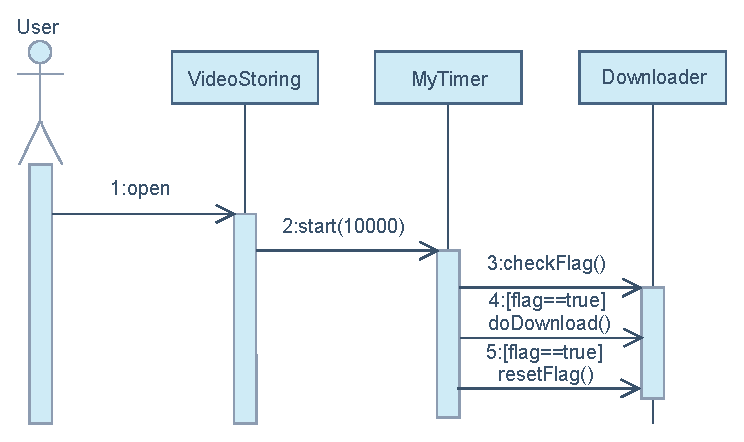
\includegraphics[width=\textwidth]{storing/sequence}
  	\caption{Video Storing: Sequence Diagram}
  	\label{Fig:sequenceStoring}
  	
  \end{figure}